\section{Mechanical Design}

\subsection{Structure \& Vehicle Layout Overview}
% Talk about key constraints drving structure and layout. Front zone, middle zone, and rear zone.

\begin{figure}[H]
\begin{minipage}[b]{0.5\linewidth}
\centering
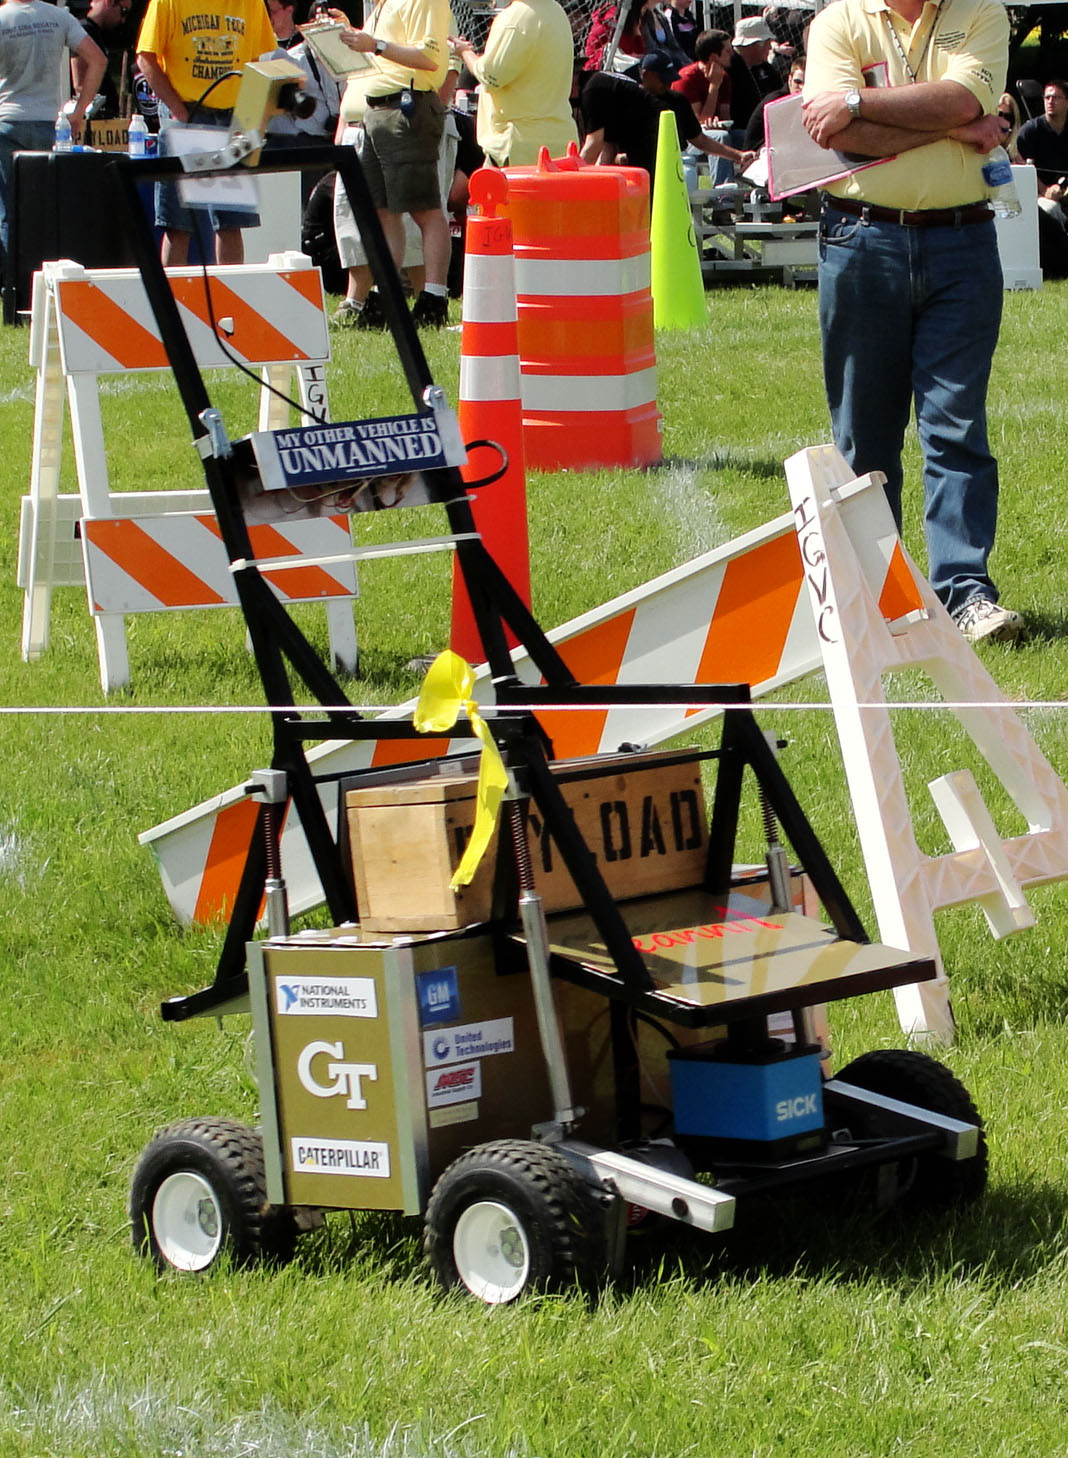
\includegraphics[width=2.5in]{./pics/2010Jeanni.jpg}
\caption{Jeanni, the 2010 base}
\label{FIG:Jeanni}
\end{minipage}
\hspace{0.1in}
\begin{minipage}[b]{0.5\linewidth}
\centering
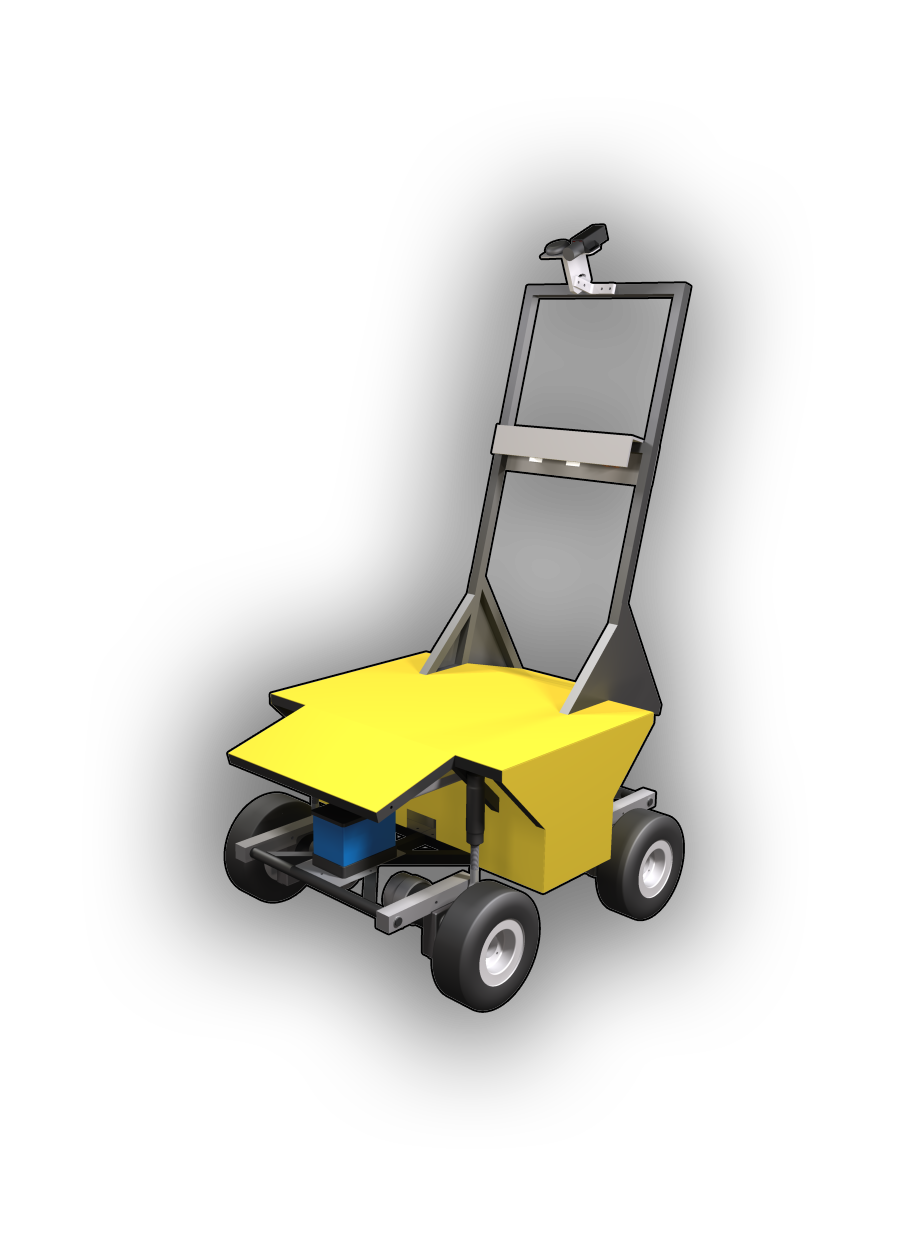
\includegraphics[width=3in]{./pics/RobotFrontCover.png}
\caption{Roxi, the 2011 Base}
\label{FIG:Trans}
\end{minipage}
\end{figure}

Following our move last year to a four wheeled drive base shown in Figure /ref{FIG:Jeanni}, our team sought to further improve on this platform which provided a large increase in maneuverability and space efficiency over our previous 2 wheeled custom ball caster model. During system debrief and review, several actionable deficiencies and areas of improvement for last years mechanical platform were noted. These included poor suspension performance, high weight, waterproofing issues, and lack of a payload restraining system that would handle the new increased speed limit. This years' drive base design, shown in Figure /ref{FIG:Roxi} was guided by the following main goals:

\begin{enumerate}
\item Increased waterproofing performance
\item Outer panel simplification
\item Reduction in overall mass
\item Improved payload accommodation
\item Ability to hold a new laptop
\item Enhanced ride characteristics for higher top speed
\end{enumerate}

To this end a new mechanical platform has been developed which features a more robust exterior panelling system, a lighter weight construction, improved electronics accommodation, and a low cost suspension. A comparison of the previous years system and the new system can be shown The previous three zone layout has been maintained with the structure being composed of a front, middle, and rear zone. Their content is as follows:

\begin{figure}[H]
\begin{center}
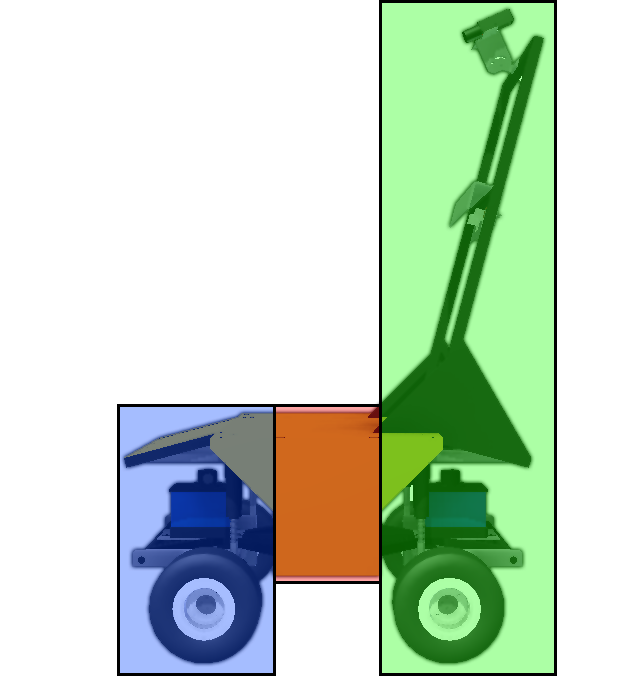
\includegraphics[width=3in]{./pics/RobotZones.png}
\caption{Robot Zones}
\label{FIG:Zones}
\end{center}
\end{figure}

\begin{enumerate}
\item \textcolor{blue}{Front}: Forward LIDAR, Motors, GPS, \& Power support for laptop
\item \textcolor{Orange}{Middle}: Main Batteries, Motor Drive Electronics, \& Power Distribution
\item \textcolor{green}{Rear}: Laptop, Camera, Rear LIDAR, GPS, Button Panel, \& Safety Light
\end{enumerate}

The frame is constructed out of 1/16" wall 1" sq. steel tube and aluminum panels. Much of the assembly was accomplished with MIG welding and the use of 1/4-20 fasteners. The outer cover is again made from polycarbonate panels which have a new attachment method that aides in rain-proofing. Overall the new system has retained many of the improvements made last year while adding key enhancements which are presented here in. 

\subsection{Drive System}
\subsubsection{Motor Configuration \& Suspension}
% We have 4 wheel independent suspension. Talk abut custom modification to off the shelf dampers.
As with last year our platform features an independently suspended four wheel drive system. Previously our suspension system was made with spare air pistons coupled with springs. These provided marginal ride smoothing, and worked well enough for our systems slow pace. In designing a new shock absorber system, our team consulted with the FormulaSAE and BajaSAE teams which we share our shop with to gain a better understanding of the shocks they utilize and what characteristics we were looking for in our system. With cost in mind we purchased some dampers for riding lawn mower seats and modified them by adding springs to their stroke. These custom shocks have become a simple yet highly costs effective solution for our needs. A close up of one of these shocks can be seen on in the CAD rendering and picture in Figure \ref{FIG:Shock}.

\begin{figure}[H]
\begin{center}
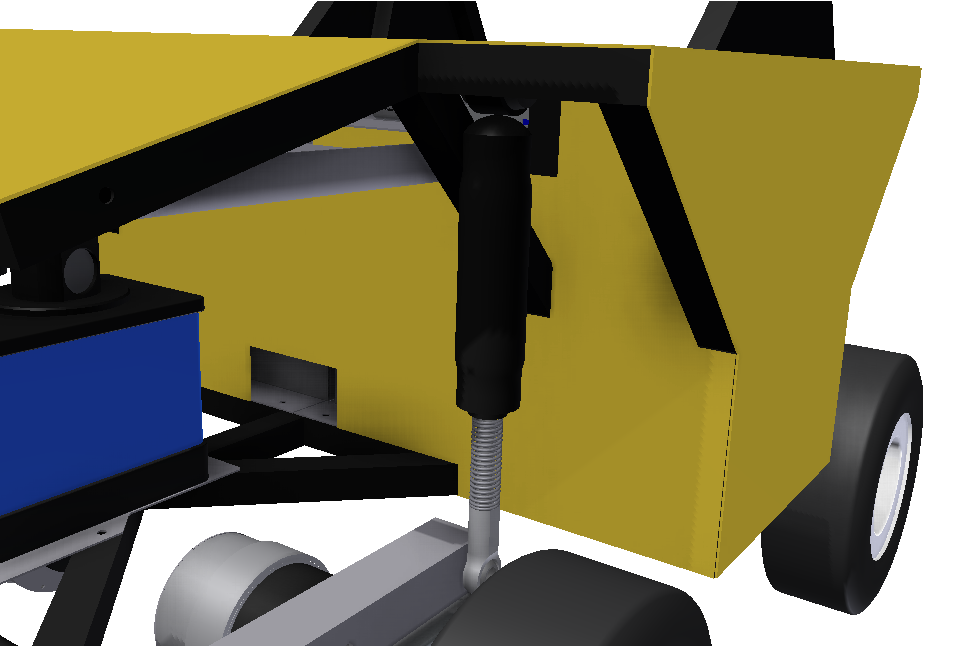
\includegraphics[width=3in]{./pics/shock.png}
\caption{Shock System}
\label{FIG:Shock}
\end{center}
\end{figure}

\subsubsection{Motor \& Encoder Modification}
% Motor specs and part number of encoders. How we mounted encoders.
As with last year, this years base is powered by four NPC T64 brushed motors. Each motor has a custom adapter plate and shaft mounted on the rear for attaching a US Digital encoder. These encoders allow for independent control of each motor by the electronics system presented later in this paper. Figure \ref{FIG:motorencoder} shows the rear of a modified motor with the attached encoder.

\begin{figure}[H]
\begin{center}
\includegraphics[width=3in]{./pics/motorencoder.png}
\caption{Motor \& Encoder Closeup}
\label{FIG:motorencoder}
\end{center}
\end{figure}

In all the T64 motors coupled with foam filled wheels allow our platform to be more than capable of handling ramps and muddy segements of the couse often encountered after rain storms during competition. 

\subsection{Waterproofing}
% Discuss waterproofing method with outter panel reduced complexity.

\subsection{Electronics Accommodation}
\subsubsection{Laptop}
% Talk about new laptop size and how it fits. Expasion on previous design. Ease of access, etc.
One of the biggest improvement to our system this year is a new laptop which moved us from our 6 year old Pentium M powered laptop to an i7 powered machine. This new laptop is larger than the previous one which prompted a reworking of the front and rear. In the end the previous year direct desk style access was attained. This year side panels were added around the laptop to reduce sun glare and enhance screen readability during field testing. The improved usability of this area and previously mentioned rain-proofing have add much to the system.

\subsubsection{Camera}
% talk about camera mounting location and field of view.

\subsubsection{LIDAR}
% Mention LIDAR FOV protection from rain, accessibility. How it comes off with 3 bolts, etc.
The modified SICK NAV 200 LIDARs are mounted in the front and rear of the vehicle and each have an unobstructed sweep of roughly 255 degrees. The LIDARs are protected above from rain by overhangs which also serve as compartments for the laptop and laptop power system. The units are attached to the base through an intermediate aluminum plate. This allows them to be removed from the vehicle with only loosening three 1/4-20 bolts which are the standard fastener for our platform.

\subsubsection{Interface Panel}
% Person based hight of interface panel. Not too high not to low, but not in the way of using the laptop.

\subsubsection{Power Electronics}
% talk about the central zone how these are held there in a compact space efficient waterproof environment.
